\documentclass[resume]{subfiles}


\begin{document}
\section{Autres}
\subsection{Triangle de Pascal}
\begin{center}
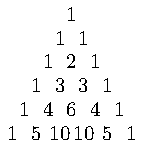
\includegraphics[scale=1,page=1]{drwg_1.pdf}
\end{center}
$$(a+b)^3=a^3+3a^2b+3ab^2+b^3$$
$$(a+b)^n=\sum_{k=0}^{n}\begin{pmatrix}
n\\k
\end{pmatrix}x^ky^{n-k}$$

$$\begin{pmatrix}
n\\ k
\end{pmatrix}=C^{n}_{k}=\frac{n!}{k!(n-k)!}$$
\subsection{Matrices}
\subsubsection{Inverses}
$$\begin{pmatrix}
\textcolor{RoyalBlue}{a} & \textcolor{OrangeRed}{b} & \textcolor{ForestGreen}{c}\\
0 & \textcolor{Violet}{d} & \textcolor{Orange}{e}\\
0 & 0 & \textcolor{ProcessBlue}{f}
\end{pmatrix}^{-1}=\begin{pmatrix}
\frac{1}{\textcolor{RoyalBlue}{a}} & -\frac{\textcolor{OrangeRed}{b}}{\textcolor{RoyalBlue}{a}\textcolor{Violet}{d}} & \frac{\textcolor{OrangeRed}{b}\textcolor{Orange}{e}-\textcolor{ForestGreen}{c}\textcolor{Violet}{d}}{\textcolor{RoyalBlue}{a}\textcolor{Violet}{d}\textcolor{ProcessBlue}{f}}\\
0 & \frac{1}{\textcolor{Violet}{d}} & -\frac{\textcolor{Orange}{e}}{\textcolor{ProcessBlue}{f}\textcolor{Violet}{d}}\\
0 & 0 & \frac{1}{\textcolor{ProcessBlue}{f}}
\end{pmatrix}$$
Même principe si on renverse
$$\left(M^{T}\right)^{-1}=\left(M^{-1}\right)^{T}$$

$$\begin{pmatrix}
\textcolor{RoyalBlue}{a} & 0 & 0\\
\textcolor{OrangeRed}{b} & \textcolor{Violet}{d} & 0\\
\textcolor{ForestGreen}{c} & \textcolor{Orange}{e} & \textcolor{ProcessBlue}{f}
\end{pmatrix}^{-1}=\begin{pmatrix}
\frac{1}{\textcolor{RoyalBlue}{a}} & 0 & 0\\
-\frac{\textcolor{OrangeRed}{b}}{\textcolor{RoyalBlue}{a}\textcolor{Violet}{d}} & \frac{1}{\textcolor{Violet}{d}} & 0\\
\frac{\textcolor{OrangeRed}{b}\textcolor{Orange}{e}-\textcolor{ForestGreen}{c}\textcolor{Violet}{d}}{\textcolor{RoyalBlue}{a}\textcolor{Violet}{d}\textcolor{ProcessBlue}{f}} & -\frac{\textcolor{Orange}{e}}{\textcolor{ProcessBlue}{f}\textcolor{Violet}{d}} &
\frac{1}{\textcolor{ProcessBlue}{f}}
\end{pmatrix}$$
Pour une matrice $2\times 2$
$$\begin{pmatrix}
\textcolor{RoyalBlue}{a} & \textcolor{OrangeRed}{b}\\
\textcolor{ForestGreen}{c} & \textcolor{Violet}{d}
\end{pmatrix}^{-1}=\frac{1}{\textcolor{RoyalBlue}{a}\textcolor{Violet}{d}-\textcolor{OrangeRed}{b}\textcolor{ForestGreen}{c}}\begin{pmatrix}
\textcolor{Violet}{d} & \textcolor{OrangeRed}{-b}\\
\textcolor{ForestGreen}{-c} & \textcolor{RoyalBlue}{a}
\end{pmatrix}$$
\end{document}